\documentclass[11pt,a4paper]{article}

\usepackage[margin=2.2cm]{geometry}
\usepackage[T1]{fontenc}
\usepackage{lmodern}
\usepackage{amssymb}
\usepackage{xcolor}
\usepackage{tikz}
\usetikzlibrary{arrows.meta,positioning}
\usepackage{booktabs}
\usepackage{tabularx}
\usepackage{enumitem}
\usepackage{listings}
\usepackage[most]{tcolorbox}
\usepackage{fancyhdr}
\usepackage[colorlinks=true,linkcolor=blue!50!black,urlcolor=blue!50!black]{hyperref}

\definecolor{local}{HTML}{2E7D32}
\definecolor{cloud}{HTML}{1565C0}
\definecolor{warn}{HTML}{C62828}
\definecolor{idea}{HTML}{6A1B9A}
\definecolor{soft}{HTML}{F5F5F5}

\newtcolorbox{concept}[1]{colback=idea!4,colframe=idea!70,fonttitle=\bfseries,title={Concept: #1},breakable}
\newtcolorbox{analogy}{colback=local!5,colframe=local!70,fonttitle=\bfseries,title={Analogy},breakable}
\newtcolorbox{why}{colback=cloud!4,colframe=cloud!70,fonttitle=\bfseries,title={Why it is done this way},breakable}
\newtcolorbox{caution}{colback=warn!4,colframe=warn!70,fonttitle=\bfseries,title={Watch out},breakable}
\newtcolorbox{exercise}{colback=soft,colframe=black!50,fonttitle=\bfseries,title={Check yourself},breakable}
\newtcolorbox{quickcheck}[1]{colback=soft,colframe=black!50,fonttitle=\bfseries,title={Quick check #1 (answer in Section~\ref{sec:answers})},breakable}

\lstset{basicstyle=\ttfamily\small,backgroundcolor=\color{soft},frame=single,
        rulecolor=\color{black!25},columns=fullflexible,keepspaces=true,
        showstringspaces=false,breaklines=true}

\pagestyle{fancy}
\fancyhf{}
\lhead{\small Listen -- Learning Doc 10}
\rhead{\small Stage 1: the Foundations in Code}
\cfoot{\thepage}

\title{\textbf{Listen}\\[4pt]\large Learning Doc 10: Stage 1, the Foundations in Code\\
       \normalsize The plumbing every later part of the agent stands on, taught from zero}
\author{Implementation, stage 1 of 6}
\date{21 October 2026, revised 29 October 2026}

\begin{document}
\sloppy
\maketitle

\begin{abstract}
\noindent Docs 01--09 were design. This is the first document about real code: the agent's
foundations, built in stage 1. It is written to be read by someone who has never studied these
ideas before. Every concept starts with the problem it solves, then the idea in plain words, an
everyday analogy (and where that analogy stops being true), a step-by-step example, the real code,
the mistakes people usually make, and a short question to check yourself. The answers are at the
end. Every program output shown here is copied from a real run on the development laptop.
\end{abstract}

\tableofcontents
\newpage

% =====================================================================
\section{Before you start}\label{sec:before}
You need these ideas. Each gets a few sentences here; the sections that use them go deeper.

\begin{description}[style=nextline,leftmargin=1.2cm,itemsep=3pt]
  \item[A program and a process] A \emph{program} is files on disk. A \emph{process} is a program
        that is running: Windows gave it memory and is executing it. \texttt{listen run} starts one
        process.
  \item[The terminal] A window where you type commands (PowerShell or Git Bash). A command is a
        program name followed by \emph{arguments}: in \texttt{listen run}, \texttt{run} is the
        argument.
  \item[A Python module and package] A module is one \texttt{.py} file. A package is a folder of
        modules with an \texttt{\_\_init\_\_.py} file in it. \texttt{listen\_agent} is a package;
        \texttt{listen\_agent/core/bus.py} is a module inside it.
  \item[Function, parameter, default] \texttt{def f(x=5):} defines a function with a parameter
        \texttt{x} whose \emph{default} is 5 when the caller gives nothing.
  \item[Class and object] A class is a blueprint (``what a Book is''); an object is one thing built
        from it (``this particular book''). \texttt{self} inside a method means ``the object this
        method was called on''.
  \item[Exception] Python's way of saying ``something went wrong'': it \emph{raises} an exception
        object, and code can \emph{catch} it with \texttt{try} / \texttt{except} and carry on.
  \item[Earlier docs] Virtual environments and \texttt{pyproject.toml} (Doc~02), threads, the
        event bus and the supervisor as designs (Doc~04), logs, tests and CI (Doc~09).
\end{description}

% =====================================================================
\section{What stage 1 built}
\begin{center}
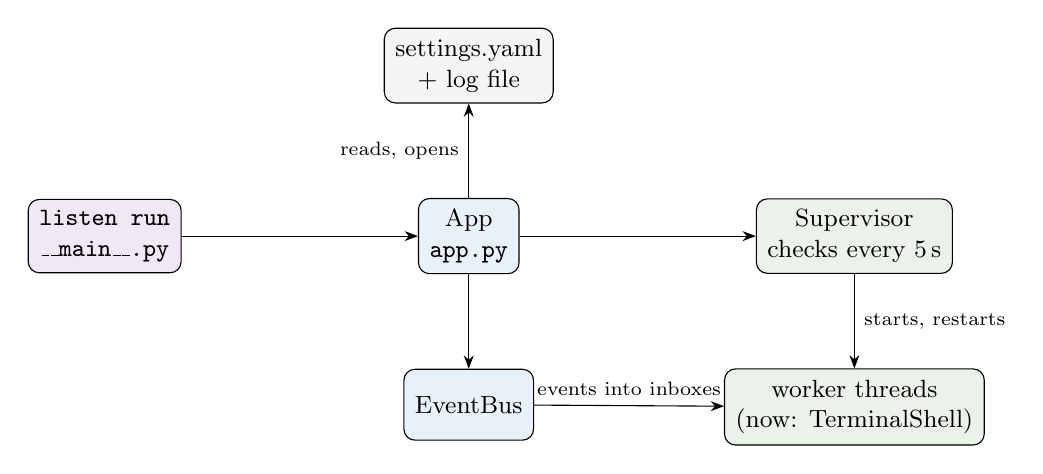
\begin{tikzpicture}[
  b/.style={draw,rounded corners,align=center,minimum height=9mm,inner sep=4pt,font=\small},
  node distance=12mm and 30mm]
  \node[b,fill=idea!10] (cli) {\texttt{listen run}\\\texttt{\_\_main\_\_.py}};
  \node[b,fill=cloud!10,right=of cli] (app) {App\\\texttt{app.py}};
  \node[b,fill=soft,above=of app] (set) {settings.yaml\\+ log file};
  \node[b,fill=local!10,right=of app] (sup) {Supervisor\\checks every 5\,s};
  \node[b,fill=cloud!10,below=of app] (bus) {EventBus};
  \node[b,fill=local!10,below=of sup] (w) {worker threads\\(now: TerminalShell)};
  \draw[-{Stealth}] (cli) -- (app);
  \draw[-{Stealth}] (app) -- node[left,font=\scriptsize]{reads, opens} (set);
  \draw[-{Stealth}] (app) -- (sup);
  \draw[-{Stealth}] (app) -- (bus);
  \draw[-{Stealth}] (sup) -- node[right,font=\scriptsize]{starts, restarts} (w);
  \draw[-{Stealth}] (bus) -- node[above,font=\scriptsize]{events into inboxes} (w);
\end{tikzpicture}
\end{center}

\noindent What happens when you type \texttt{listen run}:
\begin{enumerate}[nosep]
  \item The log file \texttt{agent/logs/listen.log} is opened.
  \item \texttt{agent/settings.yaml} is read and checked; a bad value stops here (exit code 2).
  \item The \texttt{App} creates the event bus, the workers (in stage 1 only the terminal shell)
        and the supervisor, and starts one thread per worker plus one for the supervisor.
  \item ``Listen is ready.'' is printed and logged; the main thread waits.
  \item Ctrl+C: ``Stopping\ldots'', every thread is told to stop, ``stopped'' is logged, exit code 0.
\end{enumerate}

\begin{why}
All eleven modules of stages 2--4 need settings, logging, a thread, an inbox and a way to talk to
each other. Building that once, first, and testing it alone means each later module only writes
its own job. It is also pure Python with no microphone or AI model: the gentlest place to learn
the tools.
\end{why}

% =====================================================================
\section{Installing your own package}
\subsection{The command, piece by piece}
\begin{lstlisting}
agent/.venv/Scripts/python -m pip install -e "agent[dev]"
\end{lstlisting}
\begin{center}
\renewcommand{\arraystretch}{1.15}
\begin{tabularx}{\textwidth}{l X}
\toprule
\textbf{Part} & \textbf{Meaning} \\
\midrule
\texttt{agent/.venv/} & the agent's private Python set-up (made by \texttt{python -m venv agent/.venv}) \\
\texttt{Scripts/python} & that set-up's own Python (on Linux and Mac the folder is \texttt{bin/}) \\
\texttt{-m pip} & ``run the module \texttt{pip}'': Python's package installer, the one belonging to \emph{this} Python \\
\texttt{install} & pip's subcommand (others: \texttt{uninstall}, \texttt{list}, \texttt{show}) \\
\texttt{-e} & \textbf{editable}: link to your folder instead of copying it (Section~\ref{sec:editable}) \\
\texttt{agent} & the folder holding \texttt{pyproject.toml} \\
\texttt{[dev]} & also install the optional group named \texttt{dev} (pytest and ruff) \\
\texttt{" "} & quotes stop the terminal treating \texttt{[ ]} as a file-name pattern \\
\bottomrule
\end{tabularx}
\end{center}

\begin{caution}
Spaces matter: \texttt{python-m} or \texttt{install-e} fail. And plain \texttt{pip install \ldots}
runs whichever \texttt{pip} Windows finds first, which may belong to the system Python, so the
libraries land in the wrong place. \texttt{agent/.venv/Scripts/python -m pip} cannot be ambiguous.
\end{caution}

\subsection{The format of \texttt{pyproject.toml}}
There are two layers of rules. \textbf{TOML} is the syntax: \texttt{[name]} starts a section
(a \emph{table}), \texttt{key = value} lines go inside, strings are quoted, lists use
\texttt{[ ]}, \texttt{\{ \}} is a small inline table, \texttt{\#} starts a comment, and a dotted
name like \texttt{[project.scripts]} means ``the \texttt{scripts} part inside \texttt{project}''.
\textbf{Python's packaging standards} (documents called PEPs) then fix which section names exist:
\begin{lstlisting}
[build-system]                       # PEP 518: which tool builds the package
requires = ["setuptools>=68"]
build-backend = "setuptools.build_meta"

[project]                            # PEP 621: name, Python version, dependencies
name = "listen-agent"
requires-python = ">=3.11"           # pip refuses an older Python
dependencies = ["pyyaml>=6.0"]       # ALWAYS installed: needed to RUN

[project.optional-dependencies]      # PEP 621: the "extras"
dev = ["pytest>=8.0", "ruff>=0.6"]   # installed only when you ask for [dev]

[project.scripts]
listen = "listen_agent.__main__:main"   # creates .venv/Scripts/listen.exe

[tool.ruff]                          # [tool.X]: each tool decides its own keys
line-length = 100
\end{lstlisting}

\noindent \textbf{Where \texttt{[dev]} lives:} inside \texttt{pyproject.toml}, nowhere else.
\texttt{dev} is a name we chose; Python gives it no meaning. Several groups install together with
a comma, \texttt{"agent[dev,docs]"}, and a common convention is an \texttt{all} group that points
back at the package: \texttt{all = ["listen-agent[dev,docs]"]}. Without any \texttt{[...]}, only
the main \texttt{dependencies} are installed.

\begin{caution}
Broken TOML stops pip with a parse error. A \emph{misspelt extra} is sneakier:
\texttt{"agent[dve]"} only prints a warning (``does not provide the extra'') and installs
everything \emph{except} pytest and ruff; you find out later when \texttt{pytest} is missing.
\end{caution}

\subsection{Editable or copied}\label{sec:editable}
A \textbf{normal install} copies your code into \texttt{.venv/Lib/site-packages/listen\_agent/};
edits do nothing until you reinstall. An \textbf{editable install} (\texttt{-e}) puts a signpost
there instead: ``the real code is in \texttt{Listen/agent/listen\_agent}'', so edits apply at once.

\noindent It also matters for finding files. \texttt{paths.py} starts from its own location:
\begin{lstlisting}[language=Python]
AGENT_DIR = Path(__file__).resolve().parents[2]   # two folders above paths.py's folder
\end{lstlisting}
\begin{center}
\begin{tabularx}{\textwidth}{l X X}
\toprule
\textbf{Install} & \textbf{\texttt{paths.py} lives in} & \textbf{so settings are looked for in} \\
\midrule
\texttt{-e} (ours) & \texttt{Listen/agent/listen\_agent/core/} & \texttt{Listen/agent/settings.yaml} \checkmark \\
normal & \texttt{.venv/Lib/site-packages/}\allowbreak\texttt{listen\_agent/core/} & \texttt{site-packages/settings.yaml}: missing, so defaults are used silently \\
\bottomrule
\end{tabularx}
\end{center}
\noindent We always install with \texttt{-e} while developing. When Listen is packaged as a real
app (stage 6), settings and logs will move to \texttt{\%APPDATA\%\textbackslash Listen}, next to
the database.

\subsection{What \texttt{listen.exe} is}
\texttt{[project.scripts]} makes pip write \texttt{.venv/Scripts/listen.exe}. Opened up, the real
file (108{,}386 bytes) is three parts glued together:
\begin{enumerate}[nosep]
  \item a generic \textbf{launcher program} (108{,}032 bytes), the same one inside
        \texttt{pip.exe}, \texttt{pytest.exe} and \texttt{ruff.exe};
  \item one line naming the Python to use:\\
        \texttt{\#!C:\textbackslash Users\textbackslash sanid\textbackslash \ldots\textbackslash agent\textbackslash .venv\textbackslash Scripts\textbackslash python.exe};
  \item a zipped five-line script:
\end{enumerate}
\begin{lstlisting}[language=Python]
import sys
from listen_agent.__main__ import main
if __name__ == '__main__':
    sys.argv[0] = sys.argv[0].removesuffix('.exe')
    sys.exit(main())
\end{lstlisting}
\noindent So \texttt{listen.exe} contains none of your code: it starts \emph{that} Python and calls
your \texttt{main()}, then passes its exit code back. Because the venv's path is written inside,
it always uses the right libraries; because of that same path, moving the venv breaks it (the cure
is recreating the venv and reinstalling). Reinstalling overwrites it; while the agent is running,
Windows refuses to replace it (``Access is denied''), so stop the agent first.

\subsection{PATH and activation}
\textbf{PATH} is a list of folders Windows searches, in order, when you type a bare program name;
the first match wins. \texttt{agent\textbackslash .venv\textbackslash Scripts\textbackslash
Activate.ps1} puts the venv's \texttt{Scripts} folder at the front of PATH \emph{for that window
only}. That is all activation does. A real run in a window that was \emph{not} activated:
\begin{lstlisting}
.\agent\.venv\Scripts\listen.exe --version   ->  listen 0.1.0   (exit code 0)
listen --version                             ->  not recognized (Scripts not on PATH)
\end{lstlisting}
\begin{center}
\begin{tabularx}{\textwidth}{l c X}
\toprule
\textbf{How you start it} & \textbf{Not activated} & \textbf{Why} \\
\midrule
\texttt{agent\textbackslash .venv\textbackslash Scripts\textbackslash listen.exe run} & works & full path; the exe names its Python itself \\
\texttt{agent/.venv/Scripts/python -m listen\_agent run} & works & you chose the venv's Python \\
\texttt{listen run} & fails & a bare name needs \texttt{Scripts} on PATH \\
\texttt{python -m listen\_agent run} & fails & finds the \emph{system} Python: \texttt{No module named 'yaml'} \\
\bottomrule
\end{tabularx}
\end{center}

\begin{concept}{pip + venv, uv, uvicorn and curl}
\textbf{uv} (by Astral, who also make ruff) replaces pip and venv in one very fast tool and writes
a \textbf{lock file}, \texttt{uv.lock}, recording the exact version of every library. Without one,
\texttt{ruff>=0.6} means ``whatever is newest on the day you install'', so CI can turn red after a
new release with no code change (the ``ruff is not pinned'' review finding). Stage 2 will switch
to uv. \textbf{uvicorn} is unrelated despite the name: it is the web server that will run the
FastAPI app in stage 4 (FastAPI is the kitchen, uvicorn the door and waiter).
\textbf{curl} is a command-line program for sending web requests; in Windows PowerShell type
\texttt{curl.exe}, because plain \texttt{curl} is a different PowerShell command.
\end{concept}

% =====================================================================
\section{The command line}
\begin{lstlisting}[language=Python]
def build_parser() -> argparse.ArgumentParser:
    parser = argparse.ArgumentParser(prog="listen", description="Listen voice agent")
    parser.add_argument("--version", action="version", version=f"%(prog)s {__version__}")
    commands = parser.add_subparsers(dest="command", metavar="command")
    commands.add_parser("run", help="start the agent (Ctrl+C stops it)")
    return parser

def main(argv: list[str] | None = None) -> int:
    parser = build_parser()
    args = parser.parse_args(argv)
    if args.command == "run":
        return run_agent()
    parser.print_help()
    return 0
\end{lstlisting}
\begin{itemize}[nosep]
  \item \texttt{build\_parser()} only \emph{describes} the command line: which words
        \texttt{listen} accepts. \texttt{-> argparse.ArgumentParser} is a type hint for readers.
  \item \texttt{prog} is the name in messages; \texttt{add\_subparsers(dest="command")} stores the
        chosen subcommand in \texttt{args.command}; \texttt{add\_parser("run", \ldots)} registers
        \texttt{run}.
  \item \texttt{\%(prog)s} is a placeholder filled in later by argparse. The line is formatted
        twice: the \texttt{f"..."} fills \texttt{\{\_\_version\_\_\}} now, giving
        \texttt{"\%(prog)s 0.1.0"}; argparse fills \texttt{\%(prog)s} when you type
        \texttt{-{}-version}, giving \texttt{listen 0.1.0}.
  \item \texttt{argv=None} means ``read what was typed''; tests pass a list instead.
  \item \texttt{if \_\_name\_\_ == "\_\_main\_\_"} (at the end of the file) is true only when the
        file is run, not when a test imports it.
\end{itemize}

\paragraph{\texttt{-{}-help} and \texttt{print\_help()} are not the same thing.} argparse adds
\texttt{-h/-{}-help} to every parser by itself; it prints the help and exits \emph{inside}
\texttt{parse\_args}. \texttt{print\_help()} at the end handles a different case: you typed
\texttt{listen} alone, so \texttt{args.command} is \texttt{None}. Without it, \texttt{listen}
would silently do nothing. Every path, from real runs:
\begin{center}
\begin{tabularx}{\textwidth}{l X c}
\toprule
\textbf{You type} & \textbf{What happens} & \textbf{Exit code} \\
\midrule
\texttt{listen -{}-version} & \texttt{parse\_args} prints \texttt{listen 0.1.0} and exits & 0 \\
\texttt{listen -{}-help} & \texttt{parse\_args} prints the help and exits & 0 \\
\texttt{listen run} & \texttt{return run\_agent()} & 0 / 2 / 3 \\
\texttt{listen} & falls through to \texttt{print\_help()} & 0 \\
\texttt{listen bogus} & \texttt{error: argument command: invalid choice: 'bogus'} & 2 \\
\bottomrule
\end{tabularx}
\end{center}

\subsection{Exit codes: who decided what}
\begin{center}
\begin{tabularx}{\textwidth}{c l X}
\toprule
\textbf{Code} & \textbf{Decided by} & \textbf{Meaning} \\
\midrule
0 & every program, every OS & success \\
1 & Python & an uncaught exception crashed the program \\
2 & argparse (an old Unix habit) & wrong usage: bad command or option \\
2 & \textbf{us}: \texttt{EXIT\_BAD\_SETTINGS} & fix \texttt{settings.yaml}; restarting would not help \\
3 & \textbf{us}: \texttt{EXIT\_FATAL} & crash loop or hang; the launcher (stage 2) restarts \\
\bottomrule
\end{tabularx}
\end{center}
\noindent Ours live in \texttt{app.py}. Code 2 is used twice, so a launcher could not tell ``you
typed a bad command'' from ``fix your settings''; a different number will be chosen before the
stage 2 launcher relies on it.

% =====================================================================
\section{Settings: trust a file only after checking it}
\texttt{load\_settings()} reads \texttt{settings.yaml} with \textbf{PyYAML}, the library that turns
YAML text into Python data (Python has built-in JSON and TOML readers, but no YAML one). The real
result for our file:
\begin{lstlisting}
{'hotkeys': {'continuous_toggle': 'ctrl+alt+c', 'push_to_talk': 'ctrl+alt+space'},
 'mode': 'wake',
 'thresholds': {'continuous_extra': 0.1, 'hearing': 0.6, 'high_risk_hearing': 0.75,
                'high_risk_match': 0.9, 'match': 0.75}}
\end{lstlisting}
\noindent Then every key and value is checked; a problem stops start-up with a message that starts
with the key:
\begin{lstlisting}
Can't start: threshold: unknown setting
Can't start: thresholds.match: must be a number from 0 to 1, got True
Can't start: settings.yaml: can't read it (...); save it as UTF-8
\end{lstlisting}

\begin{why}
``Ignore what you don't understand and use defaults'' sounds friendly but is the dangerous choice:
a typo like \texttt{threshold:} would silently do nothing. Fail loudly, early, and say where.
\end{why}

\begin{caution}
\textbf{Three traps, each with a test.} (1) In YAML, unquoted \texttt{yes}/\texttt{no} become
\texttt{True}/\texttt{False}, and in Python \texttt{True == 1}, so \texttt{bool} is refused
explicitly. (2) Notepad can add an invisible byte-order mark; reading with
\texttt{utf-8-sig} removes it. (3) Notepad can also save as UTF-16 or Windows-1252; those used to
crash with a raw \texttt{UnicodeDecodeError}, and now give the clear message above with exit
code 2. \textbf{Always \texttt{safe\_load}:} plain \texttt{yaml.load} can build arbitrary Python
objects from a crafted file, even run code; \texttt{safe\_load} only builds text, numbers, lists
and dicts. PyYAML also loses comments when \emph{writing}, so stage 4's web edits to command files
will use \texttt{ruamel.yaml}, which keeps them.
\end{caution}

% =====================================================================
\section{Dataclasses}\label{sec:dataclass}
\subsection{The problem}
A class that mostly \emph{holds data} needs repetitive code. A book, by hand:
\begin{lstlisting}[language=Python]
class Book:
    def __init__(self, title, pages=100):      # 1. store the values
        self.title = title
        self.pages = pages
    def __repr__(self):                        # 2. how it prints
        return f"Book(title={self.title!r}, pages={self.pages!r})"
    def __eq__(self, other):                   # 3. when two count as equal
        return (self.title, self.pages) == (other.title, other.pages)
\end{lstlisting}
\noindent Nine lines for two fields, and each new field means editing all three methods.

\subsection{The idea: let Python write them}
\begin{lstlisting}[language=Python]
@dataclass
class Book:
    title: str
    pages: int = 100
\end{lstlisting}
\noindent \texttt{@dataclass} is a \textbf{decorator}: a function that takes the class you just
wrote and returns an improved one. It reads the field list (name, type, default) and writes
\texttt{\_\_init\_\_}, \texttt{\_\_repr\_\_} and \texttt{\_\_eq\_\_}. Real output:
\begin{lstlisting}
print(Book("Atoms"))             ->  Book(title='Atoms', pages=100)
Book("Atoms") == Book("Atoms")   ->  True
\end{lstlisting}

\subsection{Option 1: \texttt{frozen=True}, read-only}
\begin{lstlisting}
f = FrozenBook("Atoms"); f.title = "x"
->  FrozenInstanceError: cannot assign to field 'title'
\end{lstlisting}
\begin{why}
One event object is put into several inboxes and read by several threads at once. If any thread
could change it, the others would see it change under them. Frozen makes that impossible; the same
goes for \texttt{Settings}, which must not change after it has been checked.
\end{why}

\subsection{Option 2: \texttt{default\_factory}, a fresh default each time}
Writing \texttt{at: datetime = datetime.now(UTC)} runs the clock \emph{once}, when the class is
defined. Real result: two events made at different moments had the \emph{same} time. The fix
hands dataclass a function to call for each new object:
\begin{lstlisting}[language=Python]
at: datetime = field(default_factory=lambda: datetime.now(UTC))   # called per object
\end{lstlisting}
\noindent Rule: if a default must be new for each object (now, an empty list, an empty dict), use
\texttt{default\_factory}. In \texttt{events.py} the function is the small named \texttt{\_now}.

\subsection{Option 3: \texttt{kw\_only=True}, solving an ordering rule}
A field without a default may not follow one with a default, because \texttt{Bad(5)} would be
ambiguous:
\begin{lstlisting}
TypeError: non-default argument 'module' follows default argument
\end{lstlisting}
\noindent That is exactly our case: the parent \texttt{Event} has \texttt{created\_at} (with a
default) and each child adds required fields. \texttt{kw\_only=True} on the parent means
``\texttt{created\_at} only by name'', so dataclass moves it to the end:
\begin{lstlisting}[language=Python]
@dataclass(frozen=True, kw_only=True)
class Event:
    created_at: datetime = field(default_factory=_now)

@dataclass(frozen=True)
class ModuleError(Event):
    module: str
    error: str

ModuleError("voice", "no mic")      # created_at filled in automatically
\end{lstlisting}

\begin{caution}
Use a dataclass when a class is mainly a named bundle of values (settings, events, a row of data).
When it is mainly behaviour (a worker, a supervisor), write a normal class.
\end{caution}

\begin{quickcheck}{1}
Why would \texttt{at: datetime = datetime.now(UTC)} give every event the same time, and what does
\texttt{default\_factory} change?
\end{quickcheck}

% =====================================================================
\section{Threads, queues and the worker loop}\label{sec:worker}
\subsection{Two prerequisites}
\begin{concept}{thread}
One line of work inside a program. Listen runs one per module, so the transcriber can work on a
recording while the listener keeps hearing. On a single processor core they take turns, and
\textbf{Windows decides when to switch}, possibly between any two steps.
\end{concept}
\begin{concept}{queue}
A \texttt{queue.Queue} is a thread-safe waiting line: one thread \texttt{put}s, another
\texttt{get}s, in order. \texttt{get(timeout=1)} waits at most one second, then raises
\texttt{queue.Empty}. Every worker owns one: its \textbf{inbox}.
\end{concept}

\subsection{The loop, line by line}
\begin{lstlisting}[language=Python]
_NOTHING = object()

def run_once(self) -> None:
    self.beat()
    try:
        message = self.inbox.get(timeout=self.wait_seconds)
    except queue.Empty:
        message = _NOTHING
    try:
        if message is _NOTHING:
            self.idle()
        else:
            self.handle(message)
    except Exception as exc:
        log.exception("%s failed handling %s", self.name, type(message).__name__)
        if not isinstance(message, ModuleError):
            self.bus.publish(ModuleError(self.name, f"{type(exc).__name__}: {exc}"))

def run(self, stop: threading.Event) -> None:
    while not stop.is_set():
        self.run_once()
\end{lstlisting}
\begin{center}
\renewcommand{\arraystretch}{1.15}
\begin{tabularx}{\textwidth}{l X}
\toprule
\textbf{Line} & \textbf{What it does and why} \\
\midrule
\texttt{\_NOTHING = object()} & a brand-new object equal to nothing else: a \textbf{sentinel} meaning ``no message''. \texttt{None} cannot play this role because \texttt{None} can be a real message. \\
\texttt{run\_once} & one pass of the loop, so tests can run exactly one pass without threads \\
\texttt{self.beat()} & record the heartbeat first, so even an idle worker beats every pass \\
\texttt{inbox.get(timeout=...)} & take the next message, waiting at most \texttt{wait\_seconds}. Waiting forever would never notice \texttt{stop} and never beat. \\
\texttt{except queue.Empty} & that is how the queue says ``nothing came''; store the sentinel \\
\texttt{if message is \_NOTHING} & \texttt{is} asks ``the very same object?'', right for a sentinel; \texttt{==} asks ``equal value?'' \\
\texttt{self.idle()} & periodic work, such as ``has the default microphone changed?'' \\
\texttt{self.handle(message)} & the module's real job, written by each module \\
\texttt{except Exception as exc} & any normal error is caught here, so one bad message cannot kill the thread \\
\texttt{log.exception(...)} & an ERROR line \emph{plus the traceback} in the log; only the message's \emph{type} is logged, never its contents \\
\texttt{if not isinstance(...)} & the brake against the error storm (Section~\ref{sec:storm}) \\
\texttt{publish(ModuleError(...))} & tell the rest of Listen, e.g.\ the terminal shows \texttt{error in voice: OSError: no mic} \\
\texttt{while not stop.is\_set()} & \texttt{stop} is a shared on/off flag (\texttt{threading.Event}); setting it ends every loop within about a second \\
\bottomrule
\end{tabularx}
\end{center}

\paragraph{The pattern} appears in almost every background worker, in any language:
\emph{loop until told to stop: wait for work but not forever; nothing came, do routine checks;
work came, do it; it failed, record it, report it, keep going.}

\subsection{Example: the same pattern with only the standard library}
A \texttt{Doubler} worker with the same \texttt{run\_once}/\texttt{run}; its \texttt{handle} prints
\texttt{message * 2}. Messages \texttt{4}, \texttt{None}, \texttt{"ab"}. Real output:
\begin{lstlisting}
double of 4 is 8
error, but still running: TypeError        <- None * 2 fails
double of ab is abab                       <- the next message still works
idle passes: 4 | thread alive: False       <- stopped cleanly when asked
\end{lstlisting}

\subsection{How a stage 2 module will use it}
A module inherits the loop and only writes its job:
\begin{lstlisting}[language=Python]
class Feedback(Worker):
    name = "feedback"
    def __init__(self, bus):
        super().__init__(bus)                     # inbox, heartbeat, loop
        bus.subscribe(CommandExecuted, self.inbox)
    def handle(self, message):
        winsound.PlaySound("done.wav", winsound.SND_FILENAME)
\end{lstlisting}

\paragraph{Daemon threads.} Workers start with \texttt{daemon=True}: when the main program ends,
they end with it, so a truly stuck thread cannot stop Listen from exiting.

\begin{quickcheck}{2}
Why does \texttt{get} use a one-second timeout instead of waiting forever for a message? Give two
reasons.
\end{quickcheck}

% =====================================================================
\section{Errors inside workers}
\subsection{\texttt{Exception} versus \texttt{BaseException}}
\texttt{except Exception} catches ordinary errors (\texttt{ValueError}, \texttt{OSError} \ldots)
but not \texttt{BaseException}s such as \texttt{SystemExit} and \texttt{KeyboardInterrupt}. Those
escape, the thread dies (logged with its traceback), and the supervisor replaces it
(Section~\ref{sec:supervisor}). Catching \emph{everything} would also swallow ``please exit''.

\subsection{Never put words you heard into an exception message}
Anything in an exception message reaches \texttt{listen.log} (through \texttt{log.exception}) and
the terminal (through \texttt{ModuleError}). Logs get attached to bug reports and pasted into
GitHub issues, so the privacy rule (spec 9.2) is: no spoken words in logs.
\begin{lstlisting}[language=Python]
raise IntentError(f"no command matches '{text}'")    # BAD: your sentence ends up in the log
raise IntentError("no command matches")              # good: what went wrong, not what was said
raise SlotError(f"{{app}} slot: unknown app ({len(value)} characters)")   # a size is fine
\end{lstlisting}
\noindent \textbf{Python itself does this}, real output:
\begin{lstlisting}
int("open vs code")              ->  invalid literal for int() with base 10: 'open vs code'
{}["search what is an atom"]     ->  KeyError: 'search what is an atom'
\end{lstlisting}
\noindent So code that handles your sentences checks before converting, or replaces the message:
\begin{lstlisting}[language=Python]
try:
    number = int(word)
except ValueError:
    raise SlotError("{number} slot: not a number") from None   # drop the original message
\end{lstlisting}
\noindent Words \emph{are} allowed on your own screen (the terminal), in the private local
database, and in the log only through \texttt{words()} with debug on.

\subsection{The error storm, and why errors are still published}\label{sec:storm}
The terminal shell listens to \emph{every} event, \texttt{ModuleError} included. If printing ever
fails (console closed), the generic worker rule fires: the shell fails, publishes a
\texttt{ModuleError}, receives it, fails to print that, publishes another\ldots{} The review measured
about 100{,}000 a second, enough to rotate away the whole log. Why not just stop publishing errors?
\begin{center}
\renewcommand{\arraystretch}{1.15}
\begin{tabularx}{\textwidth}{p{3.6cm} X X}
\toprule
\textbf{Option} & \textbf{For} & \textbf{Against} \\
\midrule
Never publish (log only) & simplest; no storm & errors invisible until you open the log; nothing can react (pop-up, red tray icon) \\
Always publish (original) & everything visible & the storm \\
\textbf{Publish, except when failing on a \texttt{ModuleError}} (chosen) & visible; loop impossible; one line in the shared loop protects every future module & that one failure goes only to the log, which loses nothing: if printing is broken it could not be shown anyway \\
Rate limit & also stops other floods & more code; still floods at the limit; drops real errors \\
Fix only the shell & targeted & future modules that listen to errors could repeat the bug \\
\bottomrule
\end{tabularx}
\end{center}
\noindent \textbf{Lesson:} anything that both \emph{sends} a kind of message and \emph{receives}
that same kind needs a brake. Two e-mail vacation auto-replies answering each other forever is the
same bug.

\begin{quickcheck}{3}
A stage 2 matcher fails on the sentence ``call mum'' and raises
\texttt{ValueError(f"no slot for \{text\}")}. Where does ``call mum'' end up, and how should the
line be written?
\end{quickcheck}

% =====================================================================
\section{Method resolution order (MRO)}\label{sec:mro}
\subsection{Prerequisite: inheritance}
\texttt{class Dog(Animal):} reads ``a Dog is an Animal, plus whatever I write here''. The child
gets everything the parent has and may \textbf{override} (replace) any of it.
\begin{lstlisting}[language=Python]
class Animal:
    def sound(self): return "some noise"
    def legs(self):  return 4
class Dog(Animal):
    def sound(self): return "woof"
class Puppy(Dog):
    pass
\end{lstlisting}
\begin{center}
\begin{tabularx}{\textwidth}{l X X}
\toprule
\textbf{Step} & \textbf{\texttt{p.sound()}: look in} & \textbf{\texttt{p.legs()}: look in} \\
\midrule
1 & \texttt{Puppy}: no & \texttt{Puppy}: no \\
2 & \texttt{Dog}: \textbf{yes}, \texttt{"woof"}, stop & \texttt{Dog}: no \\
3 & & \texttt{Animal}: \textbf{yes}, \texttt{4}, stop \\
\bottomrule
\end{tabularx}
\end{center}
\noindent That search order is the \textbf{MRO}, and Python stores it:
\texttt{Puppy.\_\_mro\_\_} is \texttt{['Puppy', 'Dog', 'Animal', 'object']} (real output), the
family read from the child upwards. \texttt{object} is the ancestor of every class.

\begin{analogy}
Looking for a hammer: your room first, then your parents' garage, then your grandparents' shed,
and you use the first one you find. \emph{Where it breaks:} a person might pick the nicest hammer;
Python always takes the \emph{first}, which is why \texttt{Dog}'s \texttt{"woof"} wins.
\end{analogy}
\begin{caution}
A child does not copy its parents' methods. Python searches for them on every call, so changing
\texttt{Animal.legs} later changes it for every \texttt{Puppy}.
\end{caution}

\subsection{How the event bus uses the MRO}
A child is also each of its parents: \texttt{isinstance(err, Event)} is \texttt{True} for a
\texttt{ModuleError}. So the shell subscribes once, to \texttt{Event}, and receives every kind of
event, including ones invented later. \texttt{publish} walks the event's MRO and, at each class,
collects whoever subscribed to that exact class. Shell subscribed to \texttt{Event}, an ``alerts''
module to \texttt{ModuleError}; publish a \texttt{ModuleError}:
\begin{center}
\begin{tabularx}{\textwidth}{c l l X}
\toprule
\textbf{Step} & \textbf{Class} & \textbf{Subscribed} & \textbf{Delivery list} \\
\midrule
1 & \texttt{ModuleError} & alerts & [alerts] \\
2 & \texttt{Event} & shell & [alerts, shell] \\
3 & \texttt{object} & nobody & [alerts, shell] \\
\bottomrule
\end{tabularx}
\end{center}
\noindent Real run: \texttt{shell got: 1 | alerts got: 1}. Method lookup \emph{stops} at the first
match; the bus walks the \emph{whole} list and collects every match. Siblings (two children of
\texttt{Event}) are never in each other's MRO: a \texttt{Transcribed} reaches the shell but not
alerts.

\subsection{One copy, never two}
If one inbox subscribes at two levels (\texttt{Event} and \texttt{ModuleError}), a naive bus adds it
twice. Real run: naive bus 2 copies, real bus 1. One line prevents it:
\begin{lstlisting}[language=Python]
for cls in type(event).__mro__:
    for inbox in self._subscribers.get(cls, ()):
        if inbox not in inboxes:          # already on the list? skip it
            inboxes.append(inbox)
\end{lstlisting}

\begin{quickcheck}{4}
\texttt{Transcribed(Event)} and \texttt{HeardInContinuous(Transcribed)}. The shell subscribes to
\texttt{Event}; module X subscribes to both \texttt{Transcribed} and \texttt{HeardInContinuous}
with one inbox. One \texttt{HeardInContinuous} is published. Walk the MRO: how many copies do X and
the shell get?
\end{quickcheck}

% =====================================================================
\section{Race conditions and locks}\label{sec:locks}
\subsection{Two prerequisites}
Threads take turns and Windows chooses the moment of each switch. And
\texttt{counter = counter + 1} is three steps, not one: \textbf{read} the value, \textbf{add} 1,
\textbf{write} it back. A switch can land between them.

\subsection{The race, step by step}
Two threads each add 1; \texttt{counter} starts at 5; the right answer is 7.
\begin{center}
\begin{tabularx}{\textwidth}{c X X c}
\toprule
\textbf{Moment} & \textbf{Thread A} & \textbf{Thread B} & \textbf{counter} \\
\midrule
1 & reads 5 & & 5 \\
2 & \emph{(switch)} & reads 5 & 5 \\
3 & & adds 1, writes 6 & 6 \\
4 & adds 1 to the 5 it read, writes 6 & & \textbf{6} (wrong) \\
\bottomrule
\end{tabularx}
\end{center}
\noindent A's ``5'' was out of date when it wrote. That is a \textbf{race condition}: the result
depends on who gets there first. A real run, two threads adding 1{,}000 each (with a tiny pause
between read and write, to make the switch land there often):
\texttt{expected 2000, got 1000}. A race gives \emph{different} wrong answers on different runs.
If A had finished all three steps before B read, B would have read 6 and written 7: the danger is
only a switch in the \emph{middle}.

\begin{analogy}
Two people check a shared bank account at the same moment (both see Rs 500) and each deposits
Rs 100; each phone saves 500 + 100 = 600. One deposit vanished. \emph{Where it breaks:} with
threads it is one processor switching, not two people acting at once; the effect is the same.
\end{analogy}

\subsection{The lock}
A \textbf{lock} is a single key. Only the thread holding it may run the guarded code, called the
\textbf{critical section}; others wait at the door.
\begin{lstlisting}[language=Python]
lock = threading.Lock()        # ONE key, shared by every thread
with lock:                     # wait for the key, take it
    current = counter          # read
    counter = current + 1      # write
                               # leaving the block always returns the key, even on an error
\end{lstlisting}
\begin{center}
\begin{tabularx}{\textwidth}{c X X l c}
\toprule
\textbf{Moment} & \textbf{Thread A} & \textbf{Thread B} & \textbf{Key} & \textbf{counter} \\
\midrule
1 & takes key, reads 5 & & A & 5 \\
2 & \emph{(switch)} & wants key, \textbf{waits} & A & 5 \\
3 & writes 6, returns key & & nobody & 6 \\
4 & & takes key, reads 6 & B & 6 \\
5 & & writes \textbf{7}, returns key & nobody & 7 \\
\bottomrule
\end{tabularx}
\end{center}
\noindent Real run with the lock: \texttt{expected 2000, got 2000}.

\begin{caution}
(1) Every piece of code that touches the shared thing must use the \emph{same} lock. (2) Creating
the lock inside the loop (\texttt{with threading.Lock():}) gives every pass its own key, so nobody
ever waits and nothing is protected; \texttt{EventBus} makes \texttt{self.\_lock} once, in
\texttt{\_\_init\_\_}. (3) Do not put more inside the lock than needed (next subsection).
\end{caution}

\subsection{Keep the critical section short}
One family phone book, three people calling Mum: looking up the number takes seconds, the call
takes minutes. Holding the book for the whole call makes the others queue for nothing; copying
the number, putting the book back, then calling lets everyone call at once. The same in code,
three threads, each copying from a shared dict and then doing 0.5\,s of slow work. Real run:
\begin{lstlisting}
call_holding_the_notebook    3 people done in 1.50 s    <- slow work inside the lock
call_after_copying           3 people done in 0.50 s    <- slow work after releasing it
\end{lstlisting}
\noindent \texttt{EventBus.publish} follows the second way: under the lock it only builds the
private list of inboxes, then releases the key and delivers.

\begin{quickcheck}{5}
In the phone-book run, why does the third thread finish at 1.5\,s when the slow work is inside the
lock? Say what each thread is doing during the first 0.5\,s.
\end{quickcheck}

% =====================================================================
\section{Deadlock}\label{sec:deadlock}
\subsection{What it is}
Two threads each \textbf{hold} something the other needs and each \textbf{waits} for the other to
let go. Neither does, so both wait forever: no crash, no error, just frozen. Ravi takes the pen and
wants the paper; Meena takes the paper and wants the pen:
\begin{center}
\begin{tabularx}{\textwidth}{c X X l l}
\toprule
\textbf{Moment} & \textbf{Ravi} & \textbf{Meena} & \textbf{Pen} & \textbf{Paper} \\
\midrule
1 & takes pen & & Ravi & -- \\
2 & & takes paper & Ravi & Meena \\
3 & wants paper, waits & & Ravi & Meena \\
4 & & wants pen, waits & Ravi & Meena \\
5\ldots & waiting & waiting & Ravi & Meena \\
\bottomrule
\end{tabularx}
\end{center}
\noindent A real run, with a 2-second limit on each wait so the demo ends:
\begin{lstlisting}
Ravi:  got the pen, now waiting for the paper...
Meena: got the paper, now waiting for the pen...
Ravi:  still waiting after 2 s -> STUCK
Meena: got the pen, writing
\end{lstlisting}
\noindent Ravi gave up, which put the pen down, and only then could Meena finish: the timeout
\emph{broke} the deadlock. Without it, the program would sit there forever, silently.

\paragraph{The four ingredients} must all be present: (1) things only one thread can hold;
(2) a thread keeps what it holds while waiting for more; (3) nobody can take a thing away;
(4) a \textbf{circle} of waiting. Remove any one and a deadlock is impossible.

\begin{analogy}
Two cars nose to nose on a one-lane bridge. \emph{Where it breaks:} drivers can see each other and
agree that one reverses; threads cannot see the circle at all, which is why deadlocks look like
quiet, not like errors.
\end{analogy}

\subsection{Breaking the circle}
If everyone takes the pen first, then the paper, the second person waits \emph{empty-handed} and
blocks nobody. Real run: \texttt{both finished, no timeout needed}.

\subsection{How Listen avoids it}
\begin{center}
\renewcommand{\arraystretch}{1.15}
\begin{tabularx}{\textwidth}{p{3.2cm} X X}
\toprule
\textbf{Ingredient} & \textbf{Escape route} & \textbf{In Listen} \\
\midrule
circle of waiting & take locks in one agreed order & no code holds two locks at once \\
hold while waiting & never hold a lock while waiting on something else & the bus copies, releases, then delivers \\
nothing taken away & timeouts: give up, release, retry & \texttt{get(timeout=1)}, \texttt{join(timeout=2)} \\
\emph{all else fails} & detect and restart & heartbeats, supervisor, launcher \\
\bottomrule
\end{tabularx}
\end{center}
\noindent \textbf{Why the bus delivers outside its lock.} Imagine inboxes with a size limit and a
\emph{bad} \texttt{publish} that calls \texttt{inbox.put(event)} while holding the bus lock. The
voice thread holds the lock and waits for space in the shell's full inbox; the shell would make
space, but first wants the bus lock to publish its own event. That is the pen and the paper in
disguise. Releasing the lock before \texttt{put} means the voice thread waits holding nothing.
Today inboxes have no limit, but the bus is written so adding one later cannot introduce this.

\begin{quickcheck}{6}
If Ravi and Meena both always take the pen first, can they still deadlock? Which ingredient does
that rule remove?
\end{quickcheck}

% =====================================================================
\section{The supervisor}\label{sec:supervisor}
Every 5 seconds the supervisor looks at each worker:
\begin{lstlisting}[language=Python]
if not self.threads[worker.name].is_alive():          # dead
    if not self._may_restart(worker.name, now):
        self.on_fatal(f"{worker.name} keeps crashing")  # 4th death in a minute
        return
    self._start_thread(worker)                          # new thread, same worker + inbox
elif now - worker.last_beat > HUNG_AFTER:              # alive but silent for 30 s
    self.on_fatal(f"{worker.name} stopped responding")
\end{lstlisting}
\begin{itemize}[nosep]
  \item A Python thread cannot be restarted, so a dead worker gets a \emph{new} thread running the
        \emph{same} worker; the inbox belongs to the worker, so waiting messages survive.
  \item Recent restart times are kept in a \texttt{deque} (a list cheap to trim from the front);
        times older than 60\,s are dropped; a fourth death within the minute is a crash loop.
  \item Python cannot safely kill a hung thread, so the cure is restarting the whole agent:
        \texttt{on\_fatal} sets exit code 3 and the launcher takes over.
\end{itemize}

\paragraph{Why 30 seconds and not 5?} A heartbeat is only recorded \emph{between} jobs. Some normal
jobs take seconds (Whisper transcribing, launching a heavy app, Windows briefly pausing Python).
A 5-second limit would restart Listen in the middle of transcribing your sentence: the command is
lost, the models reload, and one of the launcher's three restarts per 10 minutes is used up.
Waiting longer for a rare real hang costs little. Rule of thumb: a timeout sits well above the
longest normal case.

\paragraph{Sleep is not a hang.} On Windows, \texttt{time.monotonic} keeps counting while the
laptop sleeps, so after an hour with the lid closed every heartbeat looks an hour old. The
supervisor checks every 5\,s, so a gap of more than 30\,s between two of \emph{its own} checks means
the whole laptop slept; it logs ``clock jumped'' and refreshes every heartbeat. A really stuck
worker is still caught 30\,s later. This is why the hang tests advance the fake clock in 5\,s steps
with a check after each: a single 31\,s jump looks exactly like sleep.

% =====================================================================
\section{Dependency injection and fakes}\label{sec:di}
\subsection{The problem}
A \textbf{dependency} is anything outside your code that it relies on: the clock, the screen,
apps, files. Code that fetches them itself cannot be tested in a controlled way:
\begin{lstlisting}[language=Python]
def greeting_v1():
    hour = datetime.now().hour          # grabs the REAL clock itself
    return "Good morning" if hour < 12 else "Good evening"
\end{lstlisting}
\noindent ``At 9 am it says Good morning'' can only be tested in the morning.

\subsection{The idea: hand it in}
\begin{lstlisting}[language=Python]
def greeting_v2(now=datetime.now):      # the clock is a parameter; real clock by default
    hour = now().hour
    return "Good morning" if hour < 12 else "Good evening"
\end{lstlisting}
\begin{center}
\begin{tabularx}{\textwidth}{X c l}
\toprule
\textbf{Call} & \textbf{\texttt{now().hour}} & \textbf{Result (real run)} \\
\midrule
\texttt{greeting\_v2()} & real hour & \texttt{Good evening} \\
\texttt{greeting\_v2(lambda: datetime(2026,10,27,9,0))} & 9 & \texttt{Good morning} \\
\texttt{greeting\_v2(lambda: datetime(2026,10,27,21,0))} & 21 & \texttt{Good evening} \\
\bottomrule
\end{tabularx}
\end{center}
\noindent That is \textbf{dependency injection}: the dependency is passed in instead of grabbed.
(\texttt{lambda: X} is a one-line function that returns X.)

\begin{analogy}
A chef who cooks with whatever tomatoes you put on the counter: market tomatoes on a normal day,
practice ones during a test. \emph{Where it breaks:} a chef notices plastic tomatoes; code does not.
It uses anything that \emph{behaves} correctly, which is what makes fakes possible.
\end{analogy}
\begin{caution}
\texttt{def greeting\_v2(now=datetime.now()):}, \emph{with} brackets, calls the clock once when the
function is defined and freezes that moment as the default: the same trap as
\texttt{default\_factory} in Section~\ref{sec:dataclass}.
\end{caution}

\subsection{Fakes}
A \textbf{fake} is a simple stand-in that accepts the same calls. The shell only ever does
\texttt{out("text")}, so \texttt{lines.append} works just as well as \texttt{print}, and the test
reads the list. Listen's main fake is the clock:
\begin{lstlisting}[language=Python]
class FakeClock:
    def __init__(self, start=1000.0): self.now = start
    def __call__(self): return self.now          # clock() works, like time.monotonic()
    def advance(self, seconds): self.now += seconds   # time moves only when the test says
\end{lstlisting}
\noindent The three hang and sleep tests cover more than two hours of pretend time; real run:
\texttt{3 passed in 0.10s}.

\begin{center}
\renewcommand{\arraystretch}{1.15}
\begin{tabularx}{\textwidth}{l X X}
\toprule
\textbf{Name} & \textbf{What it is} & \textbf{Example} \\
\midrule
Real & the actual thing & \texttt{time.monotonic}, \texttt{print} \\
Fake & a working, simplified version & \texttt{FakeClock}; \texttt{lines.append} \\
Stub & returns a fixed answer, nothing more & \texttt{lambda: datetime(2026,10,27,9,0)} \\
Mock & a stand-in that records how it was called & a recorder checked with ``was it called with X?'' \\
\bottomrule
\end{tabularx}
\end{center}

\begin{caution}
\textbf{Share one fake wherever values are compared.} If the supervisor got a \texttt{FakeClock}
but the worker kept the real clock, the subtraction mixes two clocks. Real numbers: worker's
heartbeat 1{,}009{,}750.9, supervisor's ``now'' 1{,}031.0, silence $-$1{,}008{,}719.9 seconds:
the hang is never detected. Like two friends comparing an Indian watch with a New York phone:
each clock is fine, comparing them is the bug. Also: keep fakes tiny so they cannot drift from
reality, and assert on \emph{your} code's behaviour, not on the fake's.
\end{caution}

\subsection{What to inject, and what not}
Inject what is \textbf{slow, uncontrollable, or has real-world side effects}: the clock, the
screen, apps, volume, the microphone. Do not inject \texttt{len()}, \texttt{sorted()} or our own
pure functions such as the stage 2 matcher: test those directly with inputs and outputs. In
stage 2 the executor will take an \texttt{actions} object; tests pass a \texttt{FakeActions} that
records ``\texttt{launch\_app('Visual Studio Code')}'' in a list instead of opening anything.

\begin{quickcheck}{7}
In \texttt{greeting\_v2(now=datetime.now)}, why must there be no brackets after
\texttt{datetime.now}?
\end{quickcheck}

% =====================================================================
\section{pytest: tools and options}
\begin{center}
\renewcommand{\arraystretch}{1.15}
\begin{tabularx}{\textwidth}{l X}
\toprule
\textbf{Tool} & \textbf{What it does, and where we used it} \\
\midrule
fixture & prepares something a test needs; a test asks for it by naming it as a parameter (\texttt{bus}, \texttt{clock}, \texttt{stop}) \\
\texttt{yield} in a fixture & code after \texttt{yield} is clean-up (remove a log handler, set \texttt{stop}) \\
\texttt{conftest.py} & fixtures shared by every test in the folder; the fake clock lives there \\
\texttt{tmp\_path} & a fresh empty folder per test \\
\texttt{capsys} / \texttt{caplog} & capture printed text / log records \\
\texttt{monkeypatch} & replace something temporarily; undone after the test \\
\texttt{parametrize} & one test function, many inputs (8 bad settings files) \\
\texttt{pytest.raises} & passes only if the expected error is raised \\
\bottomrule
\end{tabularx}
\end{center}
\begin{center}
\begin{tabularx}{\textwidth}{l l X}
\toprule
\textbf{Option} & \textbf{Stands for} & \textbf{Effect} \\
\midrule
\texttt{-v} & \texttt{-{}-verbose} & one line per test instead of dots (\texttt{-vv}: more detail on failures) \\
\texttt{-k word} & keyword & only tests whose name matches; understands \texttt{and}, \texttt{or}, \texttt{not} \\
\texttt{-x} & \texttt{-{}-exitfirst} & stop at the first failure \\
\texttt{-{}-lf} & \texttt{-{}-last-failed} & re-run last time's failures (remembered in \texttt{.pytest\_cache/}) \\
\texttt{-{}-ff} & \texttt{-{}-failed-first} & last failures first, then the rest \\
\texttt{file.py::name} & a \emph{node id} & one test by its full address \\
\bottomrule
\end{tabularx}
\end{center}
\noindent These are pytest's own options: they work for every test file, including the server's
in stage 4. One dash with a letter is short (\texttt{-vx} combines two); two dashes with a word is
long and readable. Every task began with a test that failed for the right reason
(\texttt{ModuleNotFoundError}); a test that passes before the code exists tests nothing.

% =====================================================================
\section{Logging}
\begin{lstlisting}[language=Python]
LOG_FORMAT = "%(asctime)s %(levelname)-5s %(name)-8s %(message)s"
handler = RotatingFileHandler(log_dir / "listen.log", maxBytes=1_048_576, backupCount=5,
                              encoding="utf-8")
\end{lstlisting}
\noindent A \textbf{logger} is what code writes to (\texttt{logging.getLogger("core")}); a
\textbf{handler} decides where lines go; a \textbf{formatter} how they look (\texttt{-5s} pads to 5
characters). At 1\,MB, \texttt{listen.log} becomes \texttt{listen.log.1} and so on up to
\texttt{.5}. A real line:
\begin{lstlisting}
2026-10-21 15:09:37,732 INFO  core     ready (version 0.1.0, mode wake)
\end{lstlisting}
\noindent Anything you said is wrapped before logging:
\begin{lstlisting}[language=Python]
log.info("heard %s", words(text))     # "[words hidden]" unless debug is on
\end{lstlisting}
\noindent The debug flag is a plain module variable that starts \texttt{False} in every new
process, which is exactly ``debug lasts until restart''.

% =====================================================================
\section{ruff and CI}
\textbf{ruff} reads code without running it and reports likely mistakes; \texttt{-{}-fix} repairs
the safe ones. Families switched on: \textbf{E} style, \textbf{F} real mistakes (unused imports,
undefined names), \textbf{I} import order, \textbf{B} likely bugs (e.g.\ a list as a default
argument), \textbf{UP} old syntax a newer Python writes better.
\begin{center}
\begin{tabularx}{\textwidth}{l X X}
\toprule
& \textbf{PyCharm inspections} & \textbf{ruff} \\
\midrule
Runs & only in the IDE & terminal, CI, any editor \\
Settings & your IDE (not in the repo) & \texttt{pyproject.toml} (committed) \\
Ignorable? & yes, a squiggle & not in CI: a problem turns the check red \\
\bottomrule
\end{tabularx}
\end{center}
\noindent CI cannot run PyCharm, so ruff is the rule the project enforces (PyCharm's Ruff plugin
shows its warnings while you type). \texttt{.github/workflows/ci.yml} runs \texttt{ruff check agent}
and \texttt{pytest agent} on a fresh Windows machine on every push; the first run passed all 71
tests. \textbf{Pinned} means one exact version (\texttt{ruff==0.17.1}); ours are ranges
(\texttt{ruff>=0.6}), so a new release can add a check and turn CI red with no code change. A lock
file fixes that.

% =====================================================================
\section{Key takeaways and mental models}
\begin{center}
\renewcommand{\arraystretch}{1.2}
\begin{tabularx}{\textwidth}{l X}
\toprule
\textbf{Idea} & \textbf{Mental model} \\
\midrule
Editable install & a signpost to your folder, not a copy \\
\texttt{listen.exe} & ``start that Python, call \texttt{main()}'', with nothing of yours inside \\
Activation & only puts \texttt{Scripts} at the front of PATH, for one window \\
Settings & trust a file only after checking it; fail loudly, naming the key \\
Dataclass & a named bundle of values whose boring methods are written for you \\
Worker loop & wait (not forever), do the job, report failures, keep going \\
MRO & a list of ``who I am'', most specific first; methods use the first match, the bus uses all \\
Race condition & a switch landing in the middle of read-add-write \\
Lock & the one key to a small room; do the minimum inside, then hand it back \\
Deadlock & each holding half of what both need; never wait while holding \\
Dependency injection & tools are put on the code's counter; tests put toy ones there \\
Fake & a tiny stand-in that behaves the same for the calls that matter \\
\bottomrule
\end{tabularx}
\end{center}

% =====================================================================
\section{Glossary}
\begin{description}[style=nextline,leftmargin=1.2cm,itemsep=2pt]
  \item[argparse] Python's standard library for reading command-line arguments.
  \item[Critical section] Code only one thread may run at a time, guarded by a lock.
  \item[Daemon thread] A thread that ends automatically when the main program ends.
  \item[Dataclass] A class whose \texttt{\_\_init\_\_}, equality and printing are generated from its fields.
  \item[Deadlock] Threads each holding something another needs, all waiting forever.
  \item[Decorator] A function that takes a function or class and returns an improved one (\texttt{@dataclass}).
  \item[Dependency] Something outside your code that it relies on: clock, screen, files, apps.
  \item[Dependency injection] Passing a dependency in as a parameter instead of fetching it inside.
  \item[Editable install] \texttt{pip install -e}: the installed package points at your source folder.
  \item[Exit code] The number a program ends with; 0 is success.
  \item[Extra] An optional group of dependencies, e.g.\ \texttt{[dev]}.
  \item[Fake] A working, simplified stand-in used by tests.
  \item[Fixture] A pytest helper that prepares (and cleans up) something tests need.
  \item[Frozen] A dataclass whose fields cannot be changed after creation.
  \item[Handler / formatter] Where log lines go / how they look.
  \item[Heartbeat] A timestamp a worker updates on every loop pass, proving it is alive.
  \item[Inheritance] Building a class on another: the child gets everything the parent has.
  \item[Lock] A single shared key that lets one thread at a time into a critical section.
  \item[Lock file] A record of the exact version of every installed library.
  \item[Mock] A stand-in that records how it was called.
  \item[Monotonic clock] A clock that only moves forward; right for measuring durations.
  \item[MRO] Method resolution order: a class's family list, from itself up to \texttt{object}.
  \item[Override] A child replacing a method it inherited.
  \item[PATH] The ordered list of folders Windows searches for a bare program name.
  \item[Pinned] Fixed to one exact version.
  \item[Queue] A thread-safe waiting line; each worker's inbox.
  \item[Race condition] A bug that depends on which thread gets somewhere first.
  \item[Sentinel] A unique object used as a marker, e.g.\ ``nothing arrived''.
  \item[Stub] A stand-in that only returns a fixed answer.
  \item[Subcommand] One action of a multi-action program: \texttt{listen run}.
  \item[Thread] One line of work inside a program; threads take turns.
  \item[TOML] The configuration syntax of \texttt{pyproject.toml}.
\end{description}

% =====================================================================
\section{Practice questions}
\begin{exercise}
\begin{enumerate}
  \item \emph{(easy)} You change \texttt{settings.yaml} to \texttt{thresholds: \{ match: 80 \}}.
        What does \texttt{listen run} print, and what is the exit code?
  \item \emph{(easy)} Why does \texttt{python -m listen\_agent run} fail in a window where the
        venv is not activated, while \texttt{agent\textbackslash .venv\textbackslash
        Scripts\textbackslash listen.exe run} works?
  \item \emph{(easy)} What is \texttt{Dog.\_\_mro\_\_}, written as names?
  \item \emph{(medium)} A worker's \texttt{handle} raises \texttt{ValueError} on every message.
        Does the supervisor restart its thread? Why or why not?
  \item \emph{(medium)} Two threads only \emph{read} \texttt{Settings} after start-up. Do they
        need a lock?
  \item \emph{(medium)} \texttt{test\_app.py} uses \texttt{out=lines.append} but the real clock.
        Why is the real clock fine there but not in the supervisor tests?
  \item \emph{(harder)} Rewrite \texttt{publish} badly, with \texttt{inbox.put(event)} inside the
        \texttt{with self.\_lock:} block, and describe step by step a situation in which Listen
        freezes.
  \item \emph{(harder)} Stage 2's feedback module plays chimes with \texttt{winsound}. Sketch a
        design in which a test can check ``the done chime was played after a command ran''
        without any sound.
\end{enumerate}
\end{exercise}

% =====================================================================
\section{Answers}\label{sec:answers}
\subsection*{Quick checks}
\begin{enumerate}[label=\textbf{\arabic*.}]
  \item The default expression runs once, when the class is defined, and that single moment is
        stored and shared. \texttt{default\_factory} stores a \emph{function} and calls it for
        each new object.
  \item A worker waiting forever would never see \texttt{stop} being set, so shutdown would hang;
        and it would never record a heartbeat, so the supervisor would think it hung.
  \item Into the exception message, so into \texttt{listen.log} through \texttt{log.exception}
        and onto the terminal through \texttt{ModuleError}. Write
        \texttt{ValueError("no slot matched")}: what went wrong, not what was said.
  \item MRO: \texttt{HeardInContinuous}, \texttt{Transcribed}, \texttt{Event}, \texttt{object}.
        Step 1 adds X; step 2 finds X again and skips it; step 3 adds the shell. X gets 1 copy,
        the shell 1 copy.
  \item From 0 to 0.5\,s thread 1 holds the lock and does its slow work; threads 2 and 3 only
        wait for the key. Thread 2 works from 0.5 to 1.0\,s and thread 3 from 1.0 to 1.5\,s:
        single file, though none of them needed the lock for the slow part.
  \item No. Whoever gets the pen second waits holding nothing, so nobody blocks them. The rule
        removes the circular wait.
  \item Without brackets the parameter holds the clock \emph{function}, called afresh on each
        use. With brackets the clock is read once, when the function is defined, and that frozen
        moment becomes the default.
\end{enumerate}
\subsection*{Practice questions}
\begin{enumerate}[label=\textbf{\arabic*.}]
  \item \texttt{Can't start: thresholds.match: must be a number from 0 to 1, got 80}; exit code 2.
  \item A bare \texttt{python} finds the system Python, which has neither PyYAML nor Listen;
        \texttt{listen.exe} has the venv's Python path written inside it.
  \item \texttt{Dog}, \texttt{Animal}, \texttt{object}.
  \item No. The error is caught inside the loop and published as \texttt{ModuleError}; the thread
        stays alive and keeps beating. Only a thread that \emph{dies} is replaced.
  \item No. A race needs someone \emph{writing}; \texttt{Settings} is frozen, so nobody can.
  \item \texttt{test\_app.py} only waits up to two real seconds for a printed line; nothing in it
        depends on 30\,s passing. The supervisor tests need to simulate minutes and hours.
  \item The voice thread takes the bus lock and calls \texttt{put} on the shell's full inbox,
        waiting for space; the shell, to make space, first tries to publish and waits for the bus
        lock. Each waits for the other: deadlock.
  \item Give the module a \texttt{player} parameter defaulting to a function that calls
        \texttt{winsound}; the test passes a fake that appends the chime name to a list, then
        asserts the list is \texttt{["done"]} after a \texttt{CommandExecuted} is handled.
\end{enumerate}

\end{document}
